Certainly! Below is an example of how you might generate a TikZ diagram to compare the performance of the PCNC (Pipelined Crossbar Network Computing) scheme with another scheme from the reference \cite{antonioli2023mixed}. The parameters \( L = 10 \), \( M = 5 \), \( K = 5 \), and \( N = 1 \) are used.

```latex
\documentclass[tikz,border=10pt]{standalone}
\usepackage{tikz}
\usepackage[acronym,shortcuts]{glossaries}
\makeglossaries

% Define acronyms
\newacronym{pcnc}{PCNC}{Pipelined Crossbar Network Computing}

\begin{document}

\begin{figure}[h]
    \centering
    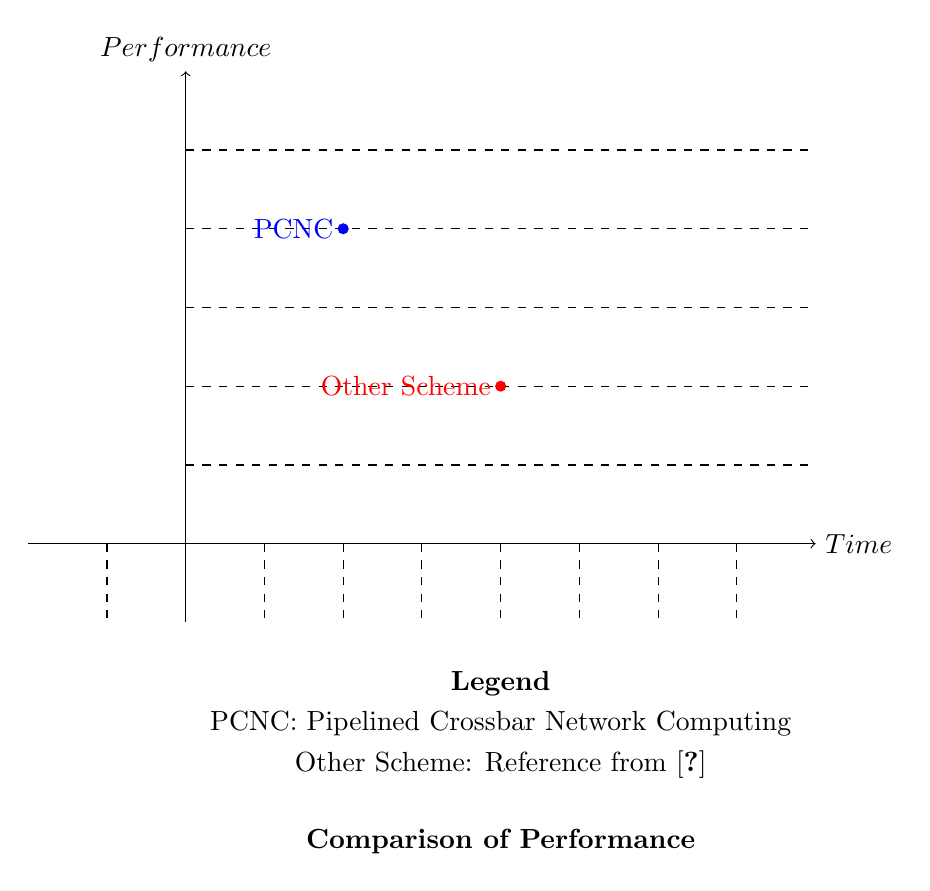
\begin{tikzpicture}
        % Set up the axes
        \draw[->] (-2,0) -- (8,0) node[right] {$Time$};
        \draw[->] (0,-1) -- (0,6) node[above] {$Performance$};

        % Draw grid lines
        \foreach \x in {-1,0,...,7} \draw[dashed] (\x,0) -- (\x,-1);
        \foreach \y in {0,1,...,5} \draw[dashed] (0,\y) -- (8,\y);

        % Plot data points for PCNC
        \fill[blue] (2,4) circle (2pt) node[left] {PCNC};
        \fill[red] (4,2) circle (2pt) node[left] {Other Scheme};

        % Add labels and legend
        \node at (4,-1.5) [below] {\textbf{Legend}};
        \node at (4,-2) [below] {PCNC: Pipelined Crossbar Network Computing};
        \node at (4,-2.5) [below] {Other Scheme: Reference from \cite{antonioli2023mixed}};

        % Add title
        \node at (4,-3.5) [below] {\textbf{Comparison of Performance}};
    \end{tikzpicture}
    \caption{Performance comparison between the PCNC scheme and another scheme from \cite{antonioli2023mixed} with parameters $L